\documentclass[../main.tex]{subfiles}
\usepackage{fancyhdr}
\graphicspath{{../images/}}

\begin{document}
\pagestyle{fancy}
\lhead{Physics 472: Li Yang}
\chead{Homework 2}
\rhead{Junseo Shin}

\renewcommand\thefigure{\arabic{figure}} 

\paragraph*{Problem 1.} Given
\begin{align*}
    M \dv[2]{u_s}{t} = C (u_{s+1} + u_{s-1} - 2u_s)
\end{align*}
where the nearest neighbors is displaced by $\pm p$ which is small so using the Taylor expansion
\begin{align*}
    u_{s + a} &\approx u_s + a \pdv{u}{x} + \frac{1}{2} a^2 \pdv[2]{u}{x} \\
    u_{s - a} &\approx u_s - a \pdv{u}{x} + \frac{1}{2} a^2 \pdv[2]{u}{x}
\end{align*} 
so
\begin{align*}
    C (u_{s+1} + u_{s-1} - 2u_s) &\approx C \qt(\cancel{u_s} + \cancel{a\pdv{u}{x}} 
        + \frac{1}{2} a^2 \pdv[2]{u}{x} + \cancel{u_s} - \cancel{a\pdv{u}{x}} +
        \frac{1}{2} a^2 \pdv[2]{u}{x} - \cancel{2u_s})
    = C a^2 \pdv[2]{u}{x}
\end{align*}
and
\begin{align*}
    M \dv[2]{u_s}{t} &= C a^2 \pdv[2]{u}{x} \\
    \dv[2]{u_s}{t} &= \frac{C a^2}{M} \pdv[2]{u}{x}
\end{align*}
since the original differential equation can have solutions with time dependence $e^{i\omega t}$
\begin{align*}
    \dv[2]{u_s}{t} &= -\omega^2 u_s
\end{align*}
and the displacements are translationally symmetric so
\begin{align*}
    u_s = ue^{iska} \qquad u_{s + 1} = ue^{i(s+1)ka} = ue^{iska}e^{ika}
    \qquad u_{s - 1} = ue^{i(s-1)ka} = ue^{iska}e^{-ika}
\end{align*}
so
\begin{align*}
    -M \omega^2 ue^{iska} &= Cue^{iska}(e^{ika} + e^{-ika} - 2) \\
    -M \omega^2 &= C(e^{ika} + e^{-ika} - 2) 
\end{align*}
where we have the trigonometric identity
\begin{align*}
    e^{ika} + e^{-ika} = 2\cosh(ika) = 2\cos(ka)
\end{align*}
so 
\begin{align*}
    -M\omega^2 &= C(2\cos(ka) - 2) \\
    \omega^2 &= \frac{2C}{M}(1 - \cos(ka))
\end{align*}
and from the half angle identity
\begin{align*}
    1 - \cos(ka) = 2\sin[2](\frac{ka}{2})
\end{align*}
so 
\begin{align*}
    \omega &= \sqrt{\frac{4C}{M}}\sin(\frac{ka}{2})
\end{align*}
we can also find the group velocity
\begin{align*}
    v &= \dv{\omega}{k} = \sqrt{\frac{4C}{M}} \cos(\frac{ka}{2}) \frac{a}{2}
        = \sqrt{\frac{Ca^2}{M}} \cos(\frac{ka}{2})
\end{align*}
and when $ka \ll 1$ or $\approx 0$, cosine is 1 so the group velocity is
\begin{align*}
    v = \sqrt{\frac{Ca^2}{M}} \qor v^2 = \frac{Ca^2}{M}
\end{align*}
so we get the wave equation
\begin{align*}
    \dv[2]{u}{t} = v^2 \dv[2]{u}{x}
\end{align*}

\paragraph*{Problem 2.} There will be two equations for alternate force constants where
the nearest neighbor for atom $u_s$ are $u'_{s}$ and $u'_{s-1}$,
and for atom $u'_s$, the nearest neights are $u_{s}$ and $u_{s+1}$. So the equations of motion are
\begin{align*}
    M \dv[2]{u}{t} &= C(u'_s - u_s) + C'(u'_{s - 1} - u_s) \\
    M \dv[2]{u'}{t} &= C' (u_{s+1} - u'_s) + C(u_{s} - u'_s)
\end{align*}
where $C' = 10 C$. The shifted parts are 
\begin{align*}
    u'_{s-1} &= u e^{iska}e^{-ika} = ue^{iska}e^{-ika} \\
    u_{s+1} &= ue^{iska}e^{ika} = ue^{iska}e^{ika}
\end{align*}
and from the previous problem $e^{iska}$ will cancel out (but not $u$ or $u'$) so 
\begin{align*}
    -M \omega^2 u &= C(u' - u) + C'(u'e^{-ika} - u) \\
    -M \omega^2 u' &= C'(ue^{ika} - u') + C(u - u')
\end{align*}
rearranging the terms for the first EQ:
\begin{align*}
    M \omega^2 u &= -C(u' - u) - C'(u'e^{-ika} - u) \\
    &= (C + C')u + (-C - C'e^{-ika})u' \\
    0&= (C + C' - M\omega^2)u + (-C - C'e^{-ika})u'
\end{align*}
and for the second EQ:
\begin{align*}
    M \omega^2 u' &= -C'(ue^{ika} - u') - C(u - u') \\
    &= (-C - C' e^{ika})u + (C + C')u' \\
    0 &= (-C - C'e^{ika})u + (C + C' - M\omega^2)u'
\end{align*}
so we have the matrix equation
\begin{align*}
    \begin{pmatrix}
        C + C' - M\omega^2 & -C - C'e^{-ika} \\
        -C - C'e^{ika} & C + C' - M\omega^2
    \end{pmatrix}
    \begin{pmatrix}
        u \\ u'
    \end{pmatrix}
    &= 0
\end{align*}
we can solve for the eigenvalues of the matrix by finding the determinant: 

\paragraph*{} For $K = 0$, the matrix is
\begin{align*}
    \begin{pmatrix}
        C + C' - M\omega^2 & -C - C' \\
        -C - C' & C + C' - M\omega^2
    \end{pmatrix}
\end{align*}
and we have a special case where $u = u'$ or
\begin{align*}
    0 &= (C + C' - M\omega^2)u + (-C - C')u = -M \omega^2  \implies \omega^2 = 0 
\end{align*}
and the other case where the determinant is zero
\begin{align*}
    0 &= (C + C' - M\omega^2)^2 - (-C - C')^2 \\
    \qusing &(a + b + c)^2 = a^2 + b^2 + c^2 + 2ab + 2bc + 2ac \\
    &= C^2 + C'^2 + M^2\omega^4 + 2CC' - 2C'M\omega^2 - 2CM\omega^2 \\
    &- (C^2 + C'^2 + 2CC') \\
    &= M^2\omega^4 - 2C'M\omega^2 - 2CM\omega^2 \\
    &= M\omega^2 - 2(C' + C)
\end{align*}
and plugging in $C' = 10C$
\begin{align*}
    0 &= M\omega^2 - 2(11C) \implies \omega^2 = 22C/M
\end{align*}
\paragraph*{} For $K = \pi/a$ and separation $a = \pi/2$ 
\begin{align*}
    e^{ika} &= e^{i\frac{\pi}{a} \frac{a}{2}} = e^{i\pi} = -1 \qquad e^{-ika} = -1 
\end{align*}
so the matrix is
\begin{align*}
    \begin{pmatrix}
        C + C' - M\omega^2 & -C + C' \\
        C - C' & C + C' - M\omega^2
    \end{pmatrix}
    \begin{pmatrix}
        u \\ u'
    \end{pmatrix}
    &= 0
\end{align*}
so for the special case where $u = u'$:
\begin{align*}
    0 &= (C + C' - M\omega^2) + (-C + C') \\
    &= 2C' - M\omega^2 \implies \omega^2 = 20C/M
\end{align*}
and the other case where the determinant is zero
\begin{align*}
    0 &= (11C - M\omega^2)^2 - (9C)^2 \\
    &= 121C^2 - 22CM\omega^2 + M^2\omega^4 - 81C^2 \\
    &= M^2\omega^4 - 22CM\omega^2 + 40C^2 \\
    &= (M\omega^2)^2 - 22C(M\omega^2) + 40C^2
\end{align*}
solving this quadratic equation where $a = 1, b = -22C, c = 40C^2$
\begin{align*}
    M\omega^2 &= \frac{22C \pm \sqrt{(-22C)^2 - 4(40C^2)}}{2} = \frac{22C \pm \sqrt{484C^2 - 160C^2}}{2} \\
    &= \frac{22C \pm \sqrt{324C^2}}{2} = \frac{22C \pm 18C}{2} = 20C, 2C
\end{align*}
so
\begin{align*}
    \omega^2 = \frac{20C}{M}, \frac{2C}{M}
\end{align*}
thus the dispersion relations are
\begin{align*}
    K&=0 : \quad \omega = 0, \sqrt{\frac{22C}{M}} \\
    K&=\pi/a : \quad \omega = \sqrt{\frac{20C}{M}}, \sqrt{\frac{2C}{M}}
\end{align*}
\begin{figure}[ht]
    \centering
    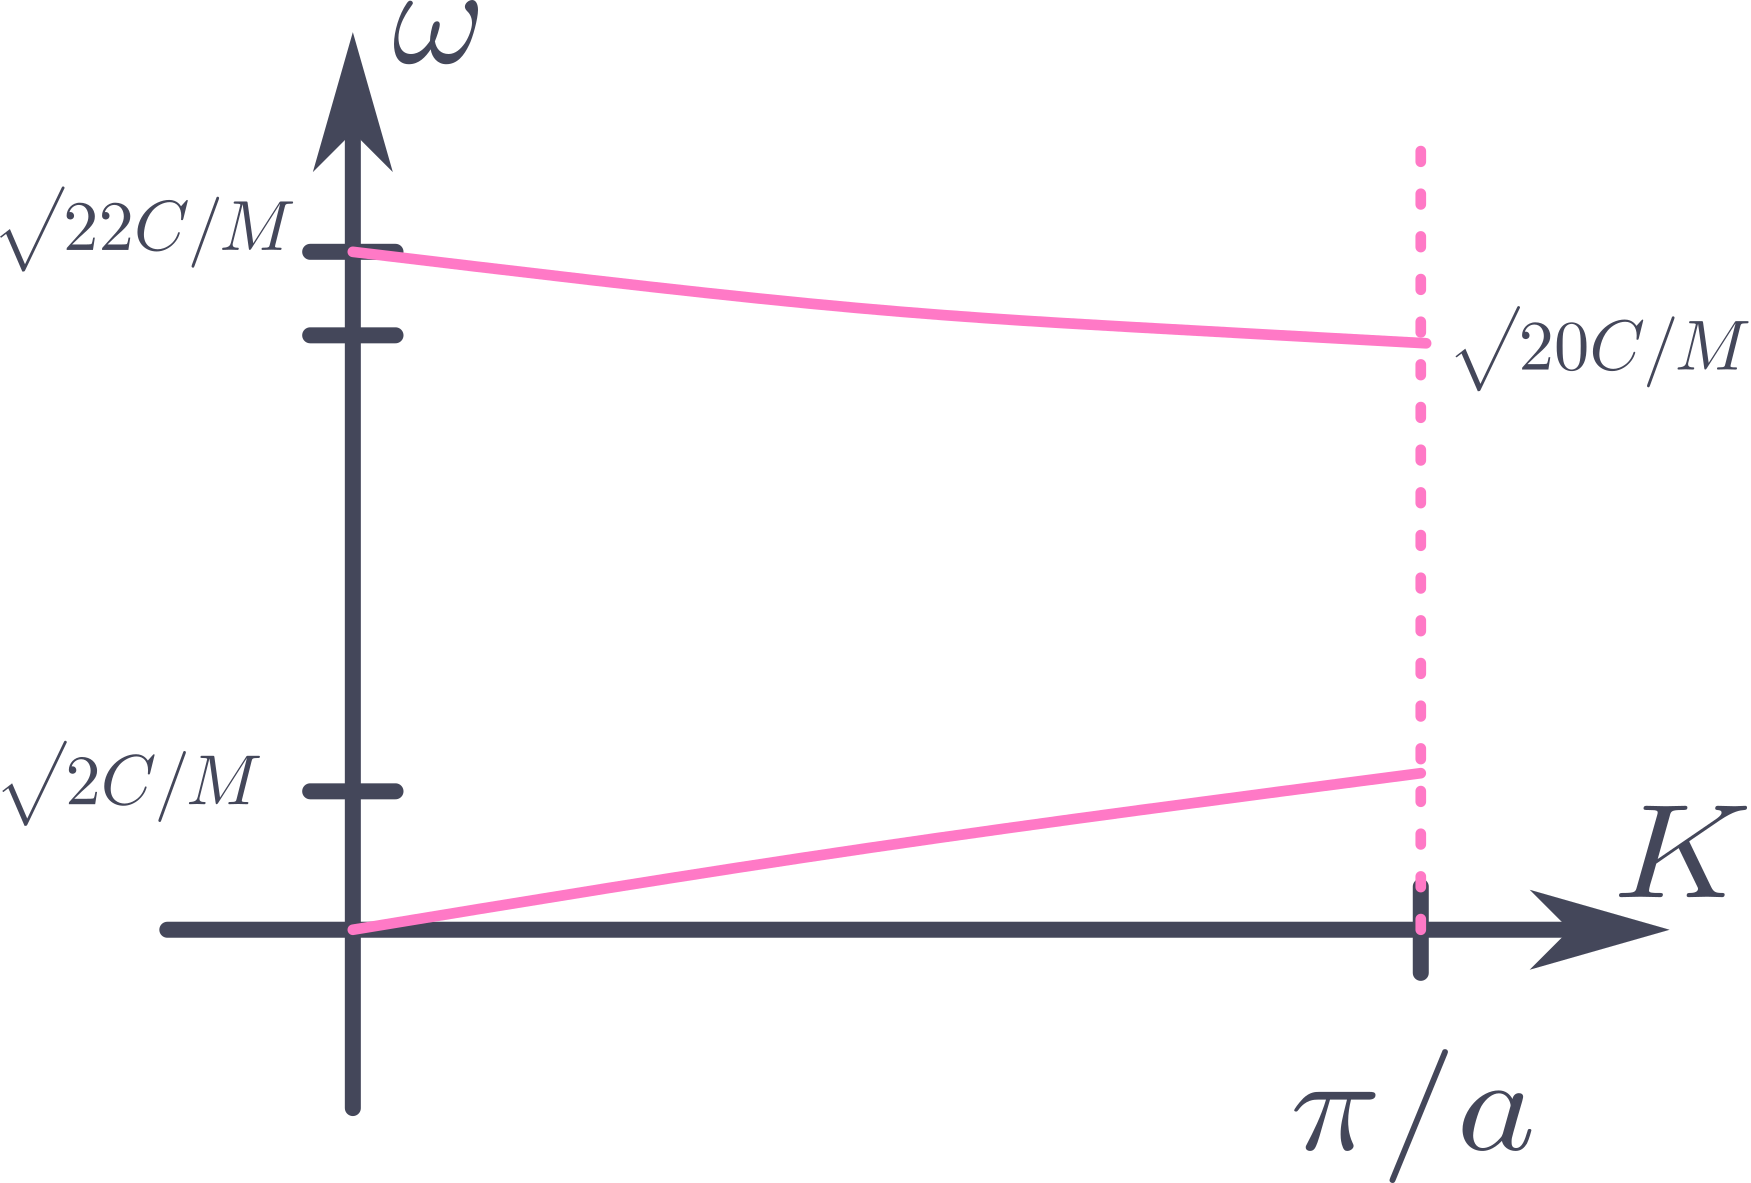
\includegraphics[width=0.5\linewidth]{hw2a.png}
    \caption{Dispersion relation for $K = 0, \pi/a$}
\end{figure}
\newpage
\paragraph*{Problem 3.} Given
\begin{align*}
    m \qt(\dv{v}{t} + \frac{v}{\tau}) &= -eE
\end{align*}
for time varying $E$ and $v$
\begin{align*}
    E = E_0 e^{-i\omega t} \qquad v = v_0 e^{-i\omega t}; \quad \dv{v}{t} = -i\omega v
\end{align*}
so solving for $v$
\begin{align*}
    m \qt(-i\omega v + \frac{v}{\tau}) &= -eE \\
    v &= \frac{-eE}{m\qt(-i\omega + \frac{1}{\tau})} \qt(\frac{\tau}{\tau})\\
    &= \frac{-eE}{m} \frac{\tau}{-i\omega\tau + 1} 
\end{align*}
from Ohm's Law 
\begin{align*}
    j = \sigma E = nqv \qor \sigma = \frac{-nev}{E} \\
    \qqtext{where} \sigma(0) = \frac{ne^2\tau}{m}
\end{align*}
where the charge is $q = -e$. Substituting $v$ from the previous equation
\begin{align*}
    \sigma &= \frac{-ne}{E} \frac{-eE}{m} \frac{\tau}{-i\omega\tau + 1} \\
    &= \frac{ne^2\tau}{m} \frac{1}{-i\omega\tau + 1}
    \qt({\frac{1 + i\omega\tau}{1 + i\omega\tau}}) \\
    \sigma(\omega) &= \sigma(0) \frac{1 + i\omega\tau}{1 + (\omega\tau)^2}
\end{align*}
where we multiply by the complex conjugate in the second step. 
\end{document}